\section{Model}
\label{sec:Model}


We consider a setting of allocating a set $M = \{1, \dots, m\}$ of indivisible items among a set $N = \{1, \dots, n\}$ of agents. 
Each agent $i \in N$ is equipped with a valuation function $v_i: 2^M \to \mathbb{R}_{\ge 0}$, and we denote by  $\boldsymbol{v} = (v_1, \dots, v_n)$ the valuation profile of all agents. 
We consider valuations that are monotone (i.e. $v(S) \le v(T)$, for all $S \subseteq T$) and normalized (v($\emptyset) = 0$). For brevity, we sometimes use $v_i(g)$ instead of $v_i(\{g\})$. 
In this work, we consider valuation classes that belong to the complement-free hierarchy, such as additive, submodular, XOS, and subadditive valuation functions which we define below.

\noindent{\bf Additive valuations.} A valuation function $v$ is additive if $v(S) = \sum_{g \in S} v(g)$ for any $S \subseteq M$.    

\noindent{\bf Submodular valuations.} A valuation function $v$ is submodular if $v(S) + v(T) \ge v(S \cup T) + v(S \cap T)$ for any $S, T \subseteq M$.    


\noindent{\bf Fractionally subadditive (XOS) valuations.} A valuation function $v$ is XOS if there exists a set of additive functions $a_1, \dots, a_k$ such that $v(S) = \max_{l \in [k]}a_l(S)$.    

\noindent{\bf Subadditive valuations.} A valuation function $v$ is subadditive if $v(S) + v(T) \ge v(S \cup T)$ for any $S, T \subseteq M$.

It is well-known that $Additive \subsetneq Submodular \subsetneq XOS \subsetneq Subadditive$.

We are interested in allocating $M$ into $n$ mutually disjoint sets $A_1,\ldots, A_n$, where $A_i$ is the bundle of items assigned to agent $i$. We denote the respective allocation by $A=(A_1, \ldots, A_n)$. 

{\bf Minimum values:} We often present to an agent a partition $P=(S_1,\ldots, S_d)$ of $M$ into $d$ parts and we ask them how they value each part. We denote by $\Pi_d(M)$ the set of all possible such partitions. We define the minimum value of agent $i$ with respect to some fixed partition $P$  as
$$\mu_i^{P}(M) = \min_{1\leq j \leq d} v_i(S_j)\,.$$
We denote by $\mu_i^{d}(M)$ the {\em maximum} minimum guarantee (MMS($d$)) that agent $i$ can achieve by the best partition with $d$ parts; i.e.,
$$\mu_i^{d}(M) = \max_{P \in \Pi_{d}(M)}\mu_i^{P}(M).$$
 We refer to the $d$ bundles $S_1,\ldots, S_d$ that comprise the best partition $P$, as the MMS$(d)$ bundles of agent $i$ or just the MMS bundles of $i$ when $d$ is clear from the context.  For $d=n$, $\mu_i^{n}(M)$ is the {\em MMS value} of agent $i$, and we drop the superscript and simply denote it by $\mu_i(M)$.  Also, when $M$ and $d$ are clear from the context, we use the simpler notation $\mu_i^{d}$ or $\mu_i$. For simplicity we assume (by scaling) that all valuations are normalized such that $\mu_i^{d}=1$. 

 Given a vector of $n$ positive integers ${\bf d}=(d_1,\ldots, d_n)$ we define a vector of partitions ${\bf P:=P(d)}=(P_1,\ldots, P_n)$ with respect to ${\bf d}$,  where the
 partition $P_i\in \Pi_{d_i}(M)$ corresponds to the partition of agent
 $i$ into $d_i$ parts. We are interested in providing
 approximation guarantees $\alpha_i$ for the minimum value
 $\mu_i^{P_i}(M)$ of each agent $i$ with respect to ${\bf P}$. This is summarised in the following definition.
\begin{definition} [$\boldsymbol{\alpha}$-MMS$(\mathbf{P})$, $\boldsymbol{\alpha}$-MMS$(\mathbf{d})$]\label{def:alpha-mms}
Fix $\boldsymbol{\alpha}=(\alpha_1,\ldots,\alpha_n)$ with $\alpha_i \in [0, 1]$, and ${\bf d}=(d_1,\ldots, d_n)$ with $d_i\in \mathbb{N}_+$ for all $i\in N$. Fix also $\mathbf{P}=(P_1,\ldots, P_n)$, a fixed vector of partitions with $P_i\in \Pi_{d_i}(M)$ for each $i$. An allocation $A$ is $\boldsymbol{\alpha}$-MMS$(\mathbf{P})$ if $v_i(A_i) \ge \alpha_i \cdot \mu_i^{P_i}(M)$ for all $i \in N$.    
An allocation $A$ is  $\boldsymbol{\alpha}$-MMS$(\mathbf{d})$ if it is $\boldsymbol{\alpha}$-MMS$(\mathbf{P(d)})$ for all partition vectors ${\bf P(d)}$ w.r.t to $\bf{d}$.\footnote{Equivalently, an allocation $A$ is  $\boldsymbol{\alpha}$-MMS$(\mathbf{d})$ if $v_i(A_i) \ge \alpha_i \cdot \mu_i^{d_i}(M)$ for all $i \in N$.}
\end{definition}

Note that for $\boldsymbol{\alpha}=(\alpha, \ldots,\alpha)$ and $\mathbf{d}=(n, \dots, n)$, the definition of $\boldsymbol{\alpha}$-MMS$(\mathbf{d})$ coincides with the standard definition of $\alpha$-MMS and we drop the dependency on $\mathbf{d}$. 
Additionally, for simplicity when $\boldsymbol{\alpha}$ is uniform, i.e., $\alpha_i=\alpha$ for each agent $i$, we write $\alpha$-MMS$(\mathbf{d})$ instead of $\boldsymbol{\alpha}$-MMS$(\mathbf{d})$. We use the notation ${\bf d}_{-i}$ and $\boldsymbol{\alpha}_{-i}$ to refer to those vectors where their $i$-th element is omitted.


\begin{figure}
\begin{center}
\small{
    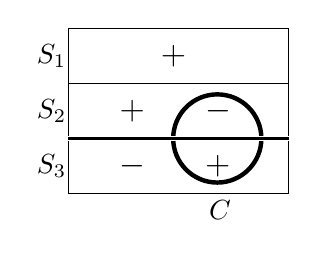
\begin{tikzpicture}[scale=0.7]
    \draw[step=1cm,] (0,-1) grid (4,2);
        \draw[left color = white, right color = white] (0,1) rectangle (4,2);
        \draw[left color = white, right color = white] (0,0) rectangle (4,1);
    \draw[left color = white, right color = white] (0,-1) rectangle (4,0);
    \draw[black,ultra thick](0.5,0) -- (3.5,0) arc(0:360:0.8) --cycle;3,0);
    \draw[white, ultra thick] (0,0) -- (4,0);
    \draw[black, thick] (0,0) -- (4,0);

\node[anchor=west] at (-0.75,1.5) {$S_1$};
\node[anchor=west] at (-0.75,0.5) {$S_2$};
\node[anchor=west] at (-0.75,-0.5) {$S_3$};
%\node[anchor=south] at (3.75,-0.75) {$C$};
\node[anchor=south] at (2.75,-1.65) {$C$};
\node[anchor=west] at (1.5,1.5) {\large{$\boldsymbol{+}$}};

\node[anchor=west] at (0.75,0.5) {\large{$\boldsymbol{+}$}};
\node[anchor=west] at (2.3,0.5) {\large{$\boldsymbol{-}$}};

\node[anchor=west] at (0.75,-0.5) {\large{$\boldsymbol{-}$}};
\node[anchor=west] at (2.3,-0.5) {\large{$\boldsymbol{+}$}};

\end{tikzpicture}}
\end{center}

    \caption{Let  $P=(S_1,S_2,S_3)$ be a partition for agent $S$. The maximum desired half over set $C$ is depicted by thick circle. For each bundle $S_i$, plus bundles (+) attain value at least  $v_S(S_i)/2$, while minus (-) attain value at most $v_S(S_i)/2$. Hence  $\mathcal{X}_{S}(C,P)=\{S_3\cap C\}$, $\mathcal{X}_{S}({M\setminus C},P)=\{S_1\setminus C,S_2 \setminus C \}$ and $\mathcal{X}^*_{S}(C,P)=\mathcal{X}_{S}({M\setminus C},P)$.}
\label{fig:maximumCut}
\end{figure}
Our allocation protocols proceed by repeatedly asking agents to
evaluate various subsets of items using specific types of valuation
queries. In the most common type of query, which we call a {\em cut}, we
present a subset $C\subseteq M$ to an agent $S$, ask her how she values
the intersection of $C$ with each of her MMS bundles $S_j$. Due to
subadditivity, at least one of $C\cap S_j$ or $C\setminus S_j$ will provide her
with satisfactory value, that is higher than $v_S(S_j)/2$. We call the side (intersection or complement) that has the highest number of satisfactory values a {\em Maximum
  Desired Half} (see definition below and Figure~\ref{fig:maximumCut} for an illustration).

\begin{definition} [Maximum Desired Half] Let $C \subseteq M$ and $P=\left(S_1,\ldots,S_r\right)\in \Pi_r(M)$ be a partition into $r$ bundles for an agent $S$. The set $\mathcal{X}_S(C,P)$ collects intersections of $C$ with each $S_i$ that have sufficiently high value (greater or equal to $1/2$) i.e.,
$$\mathcal{X}_S(C,P)=\left\{S_i \cap C : v_S\left(S_i\cap C\right)\ge \frac{v_S\left(S_i\right)}{2}, S_i \in P\right\}.$$
We define the Maximum Desired Half of agent $S$ over the set $C$ w.r.t partition $P$ as follows
$$\mathcal{X}_{S}^*(C,P) = \arg \max\left\{\lvert \mathcal{X}_S(C,P)\rvert,\lvert \mathcal{X}_S(M\setminus C,P) \rvert\right\}$$
We refer to the set $C$ as a cut $C$. When the partition $P$ is clear from the context (e.g., when the partition is the MMS bundles of $S$) we will drop the dependency on $P$.
\end{definition}

Intuitively, every bundle in the Maximum Desired Half of agent $S$
guarantees at least half the value of the minimum bundle in $P$ for
agent $S$ and moreover it is disjoint with either the cut $C$ or with
its complement w.r.t to each bundle $S_j$. The key property of the
Maximum Desired Half set is that it contains at least half of the
bundles.

\begin{observation}
\label{obs:Cut_noOfDesiredSets}
For every $C \subseteq M$ and $P=(S_1,\ldots,S_r)$, $\lvert \mathcal{X}^*_{S}(C,P)\rvert \ge \lceil r/2\rceil$.
\end{observation}
\begin{proof}
 Due to subadditivity, for each $S_i$ it holds that $v_S(S_i \cap C)+v_S(S_i \setminus C) \ge v_S(S_i)$, and therefore at least one of the two terms on the left hand side is at least $v_S(S_i)/2$, which in turn means that either $S_i\cap C \in \mathcal{X}_S(C,P)$, or $S_i \setminus C \in \mathcal{X}_S({M \setminus C},P)$ (or both). So, $\lvert {X}_S(C,P) \rvert +\lvert \mathcal{X}_S({M \setminus C},P) \rvert \ge r$ and hence, $\lvert \mathcal{X}^*_{S}(C,P)\rvert \ge r/2 \ge \lceil r/2\rceil$.   
\end{proof}


